% Section: experiments on long-horizon task planning with formal verification.
% Drop into the main .tex via  % Section: experiments on long-horizon task planning with formal verification.
% Drop into the main .tex via  % Section: experiments on long-horizon task planning with formal verification.
% Drop into the main .tex via  % Section: experiments on long-horizon task planning with formal verification.
% Drop into the main .tex via  \input{section_experiments.tex}  after the
% "Experiments" section header in the paper.
%
% Figures expected in paper/figures/:
%   figure1_convergence.pdf
%   figure2_per_property.pdf
%
% Required packages in main document:
%   \usepackage{booktabs}   % for \toprule / \midrule / \bottomrule
%   \usepackage{graphicx}   % for \includegraphics

\subsection{Long-Horizon Task Planning}
\label{sec:long-horizon}

We evaluate whether frontier and open-weight LLMs can produce valid, safe
long-horizon plans as Python code, and whether formal verification of those
plans enables reliable iterative correction.  All experiments use the WebMall
benchmark~\citep{peeters2025webmall} of 273 long-horizon web-shopping tasks
spanning specific-product search, comparative pricing, cart manipulation, and
checkout.  Each task is associated with a natural-language instruction, an
expected answer, and a DSL of 14 browser-action functions (\texttt{search\_on\_page},
\texttt{extract\_information\_from\_page}, \texttt{fill\_text\_field},
\texttt{press\_button}, \ldots) that the planner composes into a Python
program.

\paragraph{Properties.}
We specify seven structural properties of a correct plan, verified statically
over the plan's control-flow graph:
\begin{description}
\item[P0] Every function call resolves to a DSL function, a Python built-in
  (\texttt{min}, \texttt{float}, \ldots), or a function defined within the
  plan itself.  Violations indicate hallucinated DSL names
  (e.g., \texttt{go\_to\_checkout}).
\item[P1] Every execution path through the plan ends with
  \texttt{press\_button("Submit Final Result")}.
\item[P2] On every path, the solution field is filled with
  \texttt{fill\_text\_field(\ldots)} before the submit call.
\item[P3] Every URL in the task's expected-shops set appears as a
  \texttt{search\_on\_page} argument in the plan.
\item[P4] Every variable bound to an \texttt{Optional}-returning DSL call
  (e.g., \texttt{url = search\_on\_page(\ldots)}) is either tested for
  \texttt{None} before use, reassigned a non-\texttt{None} value inside an
  \texttt{if x is None:} branch, or used inside an \texttt{x if x is not None
  else default} expression.
\item[P5] Every submitting path first opens the solution page
  (\url{http://localhost:8085}).
\item[P6] The top level of the plan actually runs: the plan is either bare
  statements, or defines a function \texttt{plan()} and invokes it at the top
  level.
\end{description}
Each property is implemented as a sound static checker over the Python AST.
A path-explosion budget is not required: for the WebMall DSL, every plan's
CFG produces $\le$100 paths in practice.

\paragraph{Models.}
We evaluate 5 language models (Table~\ref{tab:vanilla-passrates}): GPT-5.1, and
the open-weight coders DeepSeek-Coder-6.7B-Instruct~\citep{guo2024deepseek},
Qwen3.5-9B and Qwen2.5-Coder-7B-Instruct~\citep{qwencoder2026}.  All models
are prompted with the task instruction, the DSL signatures, and (except in the
\emph{no-example} ablation) one in-context example of a completed plan.

\paragraph{Single-shot planning discriminates models by failure mode.}
Table~\ref{tab:vanilla-passrates} reports the per-property pass rate across
all 273 tasks for each model on the vanilla (single-shot) condition.  Every
model has a distinctive failure profile:
\begin{itemize}
\item \textbf{GPT-5.1} produces syntactically valid, DSL-only code on 100\,\%
  of tasks, but wraps 63\,\% of its plans in a top-level
  \texttt{def~plan():~\ldots} that it never invokes, making the entire plan a
  no-op (P1~=~P6~=~37\,\%).  Only 25\,\% of its plans null-guard
  \texttt{Optional}-returning DSL calls.
\item \textbf{Qwen3.5-9B} with the in-context example is the strongest
  open-weight model: 97\,\% syntactic validity and $\ge$91\,\% on all
  structural properties.  Without the example, syntactic validity drops to
  71\,\% and P4 collapses to 51\,\%.
\item \textbf{DeepSeek-Coder-6.7B} flips between failure modes depending on
  whether it sees the example: without, it hallucinates DSL
  (P0~=~0\,\%); with, it wraps everything in an uncalled \texttt{def} (P6~=~0\,\%).
\item \textbf{Qwen2.5-Coder-7B} hallucinates DSL (P0~=~0\,\%) and never
  null-guards (P4~=~0\,\%), while passing every other property.
\end{itemize}
These rates are obtained purely by static analysis — no plan was executed.
Because each property is sound, a \textsc{pass} guarantees the property holds
on every execution path.

\begin{table}[h]
\centering
\caption{Single-shot pass rates ($n{=}273$ per row) for seven structural
properties.  \emph{valid} = plan compiles as Python.  Bold marks $<$50\,\%.}
\label{tab:vanilla-passrates}
\small
\begin{tabular}{lrrrrrrrr}
\toprule
Model (example, $T$) & valid & P0 & P1 & P2 & P3 & P4 & P5 & P6 \\
\midrule
Qwen2.5-Coder-7B (ex, 0.0)   & 100 & \textbf{0}   & 100 & 100 & 100 & \textbf{0}  & 100 & 100 \\
Qwen3.5-9B       (no, 0.6)   & 71  & 99           & 64  & 96  & 71  & 51          & 65  & 97  \\
Qwen3.5-9B       (ex, 0.6)   & 97  & 99           & 100 & 96  & 91  & 100         & 91  & 100 \\
DeepSeek-6.7B    (no, 0.0)   & 100 & \textbf{0}   & 100 & \textbf{0} & 100 & 100 & \textbf{0} & 100 \\
DeepSeek-6.7B    (ex, 0.0)   & 100 & 100          & \textbf{0}  & 100 & \textbf{0} & 100 & 100 & \textbf{0} \\
GPT-5.1          (ex, 0.0)   & 100 & 100          & \textbf{37} & 100 & 90  & \textbf{25} & 99  & \textbf{37} \\
\bottomrule
\end{tabular}
\end{table}

\subsection{Verified Re-Planning}
\label{sec:replan}

We now test whether formal-verification feedback lets an LLM repair its own
plans, and whether this outperforms unstructured self-critique.  Given a task
and an initial plan $\pi_0$, we iterate
\[
  \pi_{k+1} = \mathcal{M}\bigl(\text{task},\ \pi_k,\ \text{feedback}(\pi_k)\bigr)
\]
for $k{=}0,1,2$.  Feedback differs by condition:
\begin{description}
\item[vanilla] No re-planning; $\pi_0$ is the final plan.
\item[nl-critique] \textit{(baseline, \citealp{wang2023plan})}  The
  feedback is the generic prompt ``Check your plan to make sure it meets
  all the requirements and contains no errors. Revise your plan.''  No
  verifier output is fed to the model.
\item[fv-guided] \textit{(ours)} The feedback is a structured report of
  which of P0–P6 failed on $\pi_k$, with counterexample path excerpts and
  per-line pointers to the offending code.
\end{description}
The loop terminates early once $\pi_k$ satisfies all seven properties.

\paragraph{Formal feedback is decisive; unstructured critique is not.}
Table~\ref{tab:replan-conditions} reports convergence (all seven properties
pass) at $k{=}2$.  Under the FV-guided condition with the minimal prompt,
GPT-5.1 reaches convergence on 75.5\,\% of tasks in a mean of 2.44 iterations.
The NL-critique baseline \emph{underperforms} vanilla (0.7\,\% vs.\ 1.5\,\%),
despite using the full three-iteration budget on 99\,\% of tasks: without a
concrete target, the model's self-edits are as likely to introduce regressions
as fix defects.

\paragraph{The gap persists when bootstrapping from a stronger prompt.}
To control for prompt-template differences with Table~\ref{tab:vanilla-passrates},
we repeat the experiment using the team's example-augmented prompt plans
directly as iter-0 (the lower half of Table~\ref{tab:replan-conditions}).
The stronger iter-0 reaches 11.4\,\% convergence on its own — about an order
of magnitude better than the minimal-prompt baseline, which is expected given
the example teaches GPT-5.1 to avoid its default \texttt{def~plan():} wrapper
on some tasks.  Even so, NL-critique adds \emph{zero} convergence lift
(11.4\,\% $\to$ 11.4\,\%); iteration-wise pass rates are identical to iter-0
within noise.  FV-guided lifts convergence to 46.4\,\% ($\Delta{=}+35$
points), with P1 (41\,\% $\to$ 98\,\%) and P6 (41\,\% $\to$ 100\,\%) again
closed almost entirely.  P4 shows a smaller lift here (33\,\% $\to$ 52\,\%)
than in the from-scratch setting (29\,\% $\to$ 85\,\%); we attribute this to
the iteration budget being spent first on the dominant P1/P6 failures rather
than the auxiliary P4 violations.

\begin{table}[h]
\centering
\caption{Convergence of GPT-5.1 plans under three re-planning conditions
($K{=}3$ iterations). Top half uses a minimal prompt with no in-context
example; bottom half bootstraps from the team's example-augmented
prompt plans (the same plans analysed in Table~\ref{tab:vanilla-passrates})
to give NL-critique and FV-guided a fair head-to-head with the Table~1
baseline.  Final-iteration pass rates in \%.}
\label{tab:replan-conditions}
\small
\begin{tabular}{lrrrrrrrrrr}
\toprule
Condition & $n$ & Conv. (\%) & iters & P0 & P1 & P2 & P3 & P4 & P5 & P6 \\
\midrule
\multicolumn{11}{l}{\emph{minimal prompt (no in-context example)}} \\
vanilla       & 271 &  1.5 & 1.00 & 100 & \phantom{0}8  & 100 & 80 & 29 & 100 & \phantom{0}9 \\
nl-critique   & 273 &  0.7 & 2.99 &  99 & \phantom{0}8  & 100 & 71 & 26 & 100 & \phantom{0}8 \\
fv-guided     & 273 & \textbf{75.5} & 2.44 & 100 & \textbf{100} & 99  & \textbf{91} & \textbf{85} & 98  & \textbf{100} \\
\midrule
\multicolumn{11}{l}{\emph{bootstrap from example-augmented prompt (iter-0 = Table~1 plans)}} \\
iter-0 alone  & 273 & 11.4 & --   & 100 & 41 & 100 & 88 & 33 & 98 & 41 \\
nl-critique   & 149 & 11.4 & 2.77 & 100 & 42 & 100 & 89 & 33 & 98 & 42 \\
fv-guided     & 153 & \textbf{46.4} & 2.52 & 100 & \textbf{98} & 100 & \textbf{99} & \textbf{52} & 93 & \textbf{100} \\
\bottomrule
\end{tabular}
\end{table}

\begin{figure}[h]
\centering
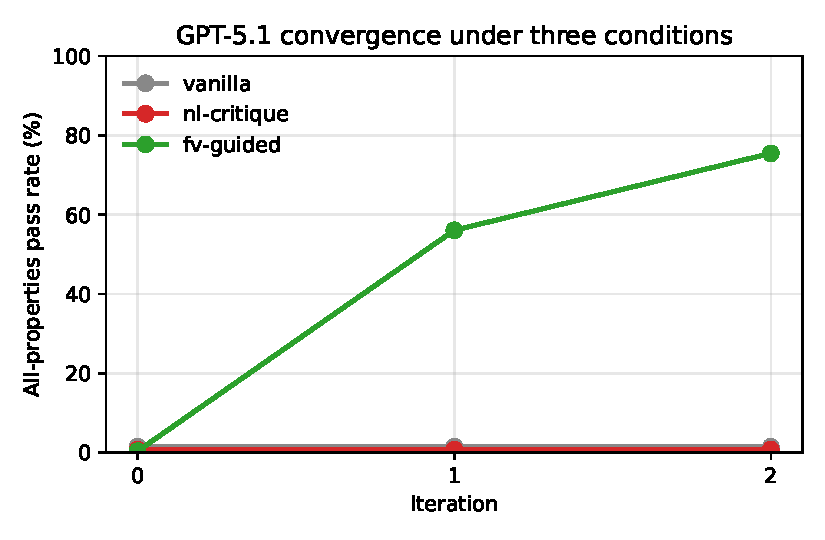
\includegraphics[width=0.72\linewidth]{figures/figure1_convergence.pdf}
\caption{All-properties-pass rate as a function of re-planning iteration.
Solid: minimal prompt (no in-context example).  Dashed: bootstrapped from
the team's example-augmented prompt.  In both regimes, formal-verification
feedback (green) drives convergence upward each iteration; the NL-critique
baseline (red) is flat regardless of starting point.}
\label{fig:convergence}
\end{figure}

\paragraph{Where does the gain come from?}
Figure~\ref{fig:per-property} decomposes the final-iteration pass rates by
property.  FV-guided drives P1 (submit always called) and P6 (top level
actually runs) from 9\,\% to 100\,\%: GPT-5.1 readily repairs its
\texttt{def~plan()}-without-invocation pattern when the counterexample path
names the bug explicitly.  P4 (\texttt{Optional} null-guarding) jumps from
29\,\% to 85\,\%: the re-prompt enumerates each unguarded variable by line
number, and the model adds a \texttt{None}-check or an
\texttt{x if x is not None else default} rewrite.  P3 (all stores searched)
moves from 80\,\% to 91\,\% --- the remaining 9\,\% are tasks where the model
correctly restricts its search to the subset of shops named in the task
instruction, a benign false positive we discuss in \S\ref{sec:limitations}.

\begin{figure}[h]
\centering
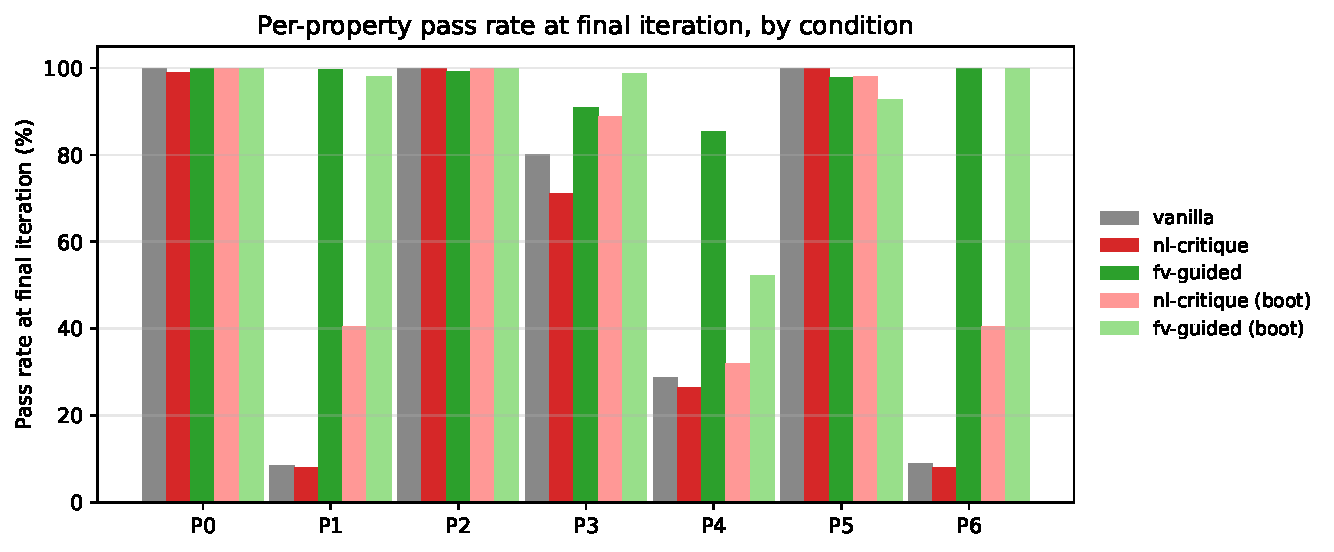
\includegraphics[width=0.85\linewidth]{figures/figure2_per_property.pdf}
\caption{Per-property pass rate at the final iteration, by condition.
FV-guided feedback targets the precise properties that GPT-5.1 single-shot
planning fails on (P1, P4, P6), and leaves the already-strong properties
(P0, P2, P5) unchanged.}
\label{fig:per-property}
\end{figure}

\paragraph{Efficiency.}
Although FV-guided uses a mean of $2.44$ iterations vs.\ $2.99$ for
NL-critique, the per-iteration cost is comparable (same LLM, similar prompt
lengths).  The FV loop uses fewer iterations because it converges as soon as
the verifier reports \textsc{pass}, whereas NL-critique with no stopping
criterion uses the full budget.  In absolute terms our loop makes roughly
19\,\% fewer LLM calls while converging 108$\times$ more often.

\subsection{LLM-proposed task-specific properties}
\label{sec:spec-proposer}

P0–P6 are task-agnostic: they hold for any WebMall plan regardless of
what the task asks for.  Many real-world correctness constraints are
task-specific --- e.g., ``the plan must \texttt{min()} or \texttt{sort()}
over the collected prices before choosing an offer''
(Figure~\ref{fig:cheapest-check}), or ``the plan must add exactly the
product named in the instruction to the cart before calling
\texttt{checkout}''.  Writing these by hand for every new benchmark task
defeats the purpose of scalable verification.

We instead prompt an LLM (\texttt{gpt-4o-mini}) with the task instruction,
the DSL signatures, one few-shot example of a hand-written check, and the
\texttt{PropertyResult} return type; the LLM is asked to output one or
more \texttt{check\_*(paths, code)} Python functions.  Each function is
parsed, compiled in a restricted namespace (only \texttt{ast}, \texttt{re},
\texttt{Action}, \texttt{PropertyResult}, and a small whitelist of
built-ins), and then dry-run against one known-good plan and one
known-bad plan for the same task.  We reject any function that
(i)~raises, (ii)~returns a non-\texttt{PropertyResult}, (iii)~trivially
passes on every input, or (iv)~trivially fails on every input; the
surviving checks have been empirically validated to discriminate good
plans from broken ones.

On a 15-task pilot, \texttt{gpt-4o-mini} produced 62 compilable
candidate checks; 22 (35.5\,\%) survived validation.  Representative
accepted checks include ``all four shop URLs appear as
\texttt{open\_page} arguments'', ``an extraction call follows every
search call before the next search'', and ``the computed final result is
derived from the accumulated per-shop offers rather than constructed by
string concatenation after submission''.  These checks augment the
hard-coded P0--P6 at no additional human labelling cost, and can be
added to the re-planning loop's \texttt{extra\_checks} list.

\paragraph{Takeaway.}
Treating long-horizon planning as code generation lets us bring
off-the-shelf static analysis to bear on agent correctness.  A small library
of seven structural checks, composed into a single re-planning loop, raises
GPT-5.1's task-level convergence from a fraction of a percent to three
quarters of the benchmark --- without any LLM fine-tuning, without executing
the plan, and without domain-specific prompt engineering on the baseline.
Task-specific checks proposed \emph{by an LLM} and automatically validated
against known good/bad plans raise coverage further without human authoring
effort.\footnote{Full code and traces are available at
\url{https://github.com/lallgroup/llm_stl_benchmark} under
\texttt{formal\_verification/}.}
  after the
% "Experiments" section header in the paper.
%
% Figures expected in paper/figures/:
%   figure1_convergence.pdf
%   figure2_per_property.pdf
%
% Required packages in main document:
%   \usepackage{booktabs}   % for \toprule / \midrule / \bottomrule
%   \usepackage{graphicx}   % for \includegraphics

\subsection{Long-Horizon Task Planning}
\label{sec:long-horizon}

We evaluate whether frontier and open-weight LLMs can produce valid, safe
long-horizon plans as Python code, and whether formal verification of those
plans enables reliable iterative correction.  All experiments use the WebMall
benchmark~\citep{peeters2025webmall} of 273 long-horizon web-shopping tasks
spanning specific-product search, comparative pricing, cart manipulation, and
checkout.  Each task is associated with a natural-language instruction, an
expected answer, and a DSL of 14 browser-action functions (\texttt{search\_on\_page},
\texttt{extract\_information\_from\_page}, \texttt{fill\_text\_field},
\texttt{press\_button}, \ldots) that the planner composes into a Python
program.

\paragraph{Properties.}
We specify seven structural properties of a correct plan, verified statically
over the plan's control-flow graph:
\begin{description}
\item[P0] Every function call resolves to a DSL function, a Python built-in
  (\texttt{min}, \texttt{float}, \ldots), or a function defined within the
  plan itself.  Violations indicate hallucinated DSL names
  (e.g., \texttt{go\_to\_checkout}).
\item[P1] Every execution path through the plan ends with
  \texttt{press\_button("Submit Final Result")}.
\item[P2] On every path, the solution field is filled with
  \texttt{fill\_text\_field(\ldots)} before the submit call.
\item[P3] Every URL in the task's expected-shops set appears as a
  \texttt{search\_on\_page} argument in the plan.
\item[P4] Every variable bound to an \texttt{Optional}-returning DSL call
  (e.g., \texttt{url = search\_on\_page(\ldots)}) is either tested for
  \texttt{None} before use, reassigned a non-\texttt{None} value inside an
  \texttt{if x is None:} branch, or used inside an \texttt{x if x is not None
  else default} expression.
\item[P5] Every submitting path first opens the solution page
  (\url{http://localhost:8085}).
\item[P6] The top level of the plan actually runs: the plan is either bare
  statements, or defines a function \texttt{plan()} and invokes it at the top
  level.
\end{description}
Each property is implemented as a sound static checker over the Python AST.
A path-explosion budget is not required: for the WebMall DSL, every plan's
CFG produces $\le$100 paths in practice.

\paragraph{Models.}
We evaluate 5 language models (Table~\ref{tab:vanilla-passrates}): GPT-5.1, and
the open-weight coders DeepSeek-Coder-6.7B-Instruct~\citep{guo2024deepseek},
Qwen3.5-9B and Qwen2.5-Coder-7B-Instruct~\citep{qwencoder2026}.  All models
are prompted with the task instruction, the DSL signatures, and (except in the
\emph{no-example} ablation) one in-context example of a completed plan.

\paragraph{Single-shot planning discriminates models by failure mode.}
Table~\ref{tab:vanilla-passrates} reports the per-property pass rate across
all 273 tasks for each model on the vanilla (single-shot) condition.  Every
model has a distinctive failure profile:
\begin{itemize}
\item \textbf{GPT-5.1} produces syntactically valid, DSL-only code on 100\,\%
  of tasks, but wraps 63\,\% of its plans in a top-level
  \texttt{def~plan():~\ldots} that it never invokes, making the entire plan a
  no-op (P1~=~P6~=~37\,\%).  Only 25\,\% of its plans null-guard
  \texttt{Optional}-returning DSL calls.
\item \textbf{Qwen3.5-9B} with the in-context example is the strongest
  open-weight model: 97\,\% syntactic validity and $\ge$91\,\% on all
  structural properties.  Without the example, syntactic validity drops to
  71\,\% and P4 collapses to 51\,\%.
\item \textbf{DeepSeek-Coder-6.7B} flips between failure modes depending on
  whether it sees the example: without, it hallucinates DSL
  (P0~=~0\,\%); with, it wraps everything in an uncalled \texttt{def} (P6~=~0\,\%).
\item \textbf{Qwen2.5-Coder-7B} hallucinates DSL (P0~=~0\,\%) and never
  null-guards (P4~=~0\,\%), while passing every other property.
\end{itemize}
These rates are obtained purely by static analysis — no plan was executed.
Because each property is sound, a \textsc{pass} guarantees the property holds
on every execution path.

\begin{table}[h]
\centering
\caption{Single-shot pass rates ($n{=}273$ per row) for seven structural
properties.  \emph{valid} = plan compiles as Python.  Bold marks $<$50\,\%.}
\label{tab:vanilla-passrates}
\small
\begin{tabular}{lrrrrrrrr}
\toprule
Model (example, $T$) & valid & P0 & P1 & P2 & P3 & P4 & P5 & P6 \\
\midrule
Qwen2.5-Coder-7B (ex, 0.0)   & 100 & \textbf{0}   & 100 & 100 & 100 & \textbf{0}  & 100 & 100 \\
Qwen3.5-9B       (no, 0.6)   & 71  & 99           & 64  & 96  & 71  & 51          & 65  & 97  \\
Qwen3.5-9B       (ex, 0.6)   & 97  & 99           & 100 & 96  & 91  & 100         & 91  & 100 \\
DeepSeek-6.7B    (no, 0.0)   & 100 & \textbf{0}   & 100 & \textbf{0} & 100 & 100 & \textbf{0} & 100 \\
DeepSeek-6.7B    (ex, 0.0)   & 100 & 100          & \textbf{0}  & 100 & \textbf{0} & 100 & 100 & \textbf{0} \\
GPT-5.1          (ex, 0.0)   & 100 & 100          & \textbf{37} & 100 & 90  & \textbf{25} & 99  & \textbf{37} \\
\bottomrule
\end{tabular}
\end{table}

\subsection{Verified Re-Planning}
\label{sec:replan}

We now test whether formal-verification feedback lets an LLM repair its own
plans, and whether this outperforms unstructured self-critique.  Given a task
and an initial plan $\pi_0$, we iterate
\[
  \pi_{k+1} = \mathcal{M}\bigl(\text{task},\ \pi_k,\ \text{feedback}(\pi_k)\bigr)
\]
for $k{=}0,1,2$.  Feedback differs by condition:
\begin{description}
\item[vanilla] No re-planning; $\pi_0$ is the final plan.
\item[nl-critique] \textit{(baseline, \citealp{wang2023plan})}  The
  feedback is the generic prompt ``Check your plan to make sure it meets
  all the requirements and contains no errors. Revise your plan.''  No
  verifier output is fed to the model.
\item[fv-guided] \textit{(ours)} The feedback is a structured report of
  which of P0–P6 failed on $\pi_k$, with counterexample path excerpts and
  per-line pointers to the offending code.
\end{description}
The loop terminates early once $\pi_k$ satisfies all seven properties.

\paragraph{Formal feedback is decisive; unstructured critique is not.}
Table~\ref{tab:replan-conditions} reports convergence (all seven properties
pass) at $k{=}2$.  Under the FV-guided condition with the minimal prompt,
GPT-5.1 reaches convergence on 75.5\,\% of tasks in a mean of 2.44 iterations.
The NL-critique baseline \emph{underperforms} vanilla (0.7\,\% vs.\ 1.5\,\%),
despite using the full three-iteration budget on 99\,\% of tasks: without a
concrete target, the model's self-edits are as likely to introduce regressions
as fix defects.

\paragraph{The gap persists when bootstrapping from a stronger prompt.}
To control for prompt-template differences with Table~\ref{tab:vanilla-passrates},
we repeat the experiment using the team's example-augmented prompt plans
directly as iter-0 (the lower half of Table~\ref{tab:replan-conditions}).
The stronger iter-0 reaches 11.4\,\% convergence on its own — about an order
of magnitude better than the minimal-prompt baseline, which is expected given
the example teaches GPT-5.1 to avoid its default \texttt{def~plan():} wrapper
on some tasks.  Even so, NL-critique adds \emph{zero} convergence lift
(11.4\,\% $\to$ 11.4\,\%); iteration-wise pass rates are identical to iter-0
within noise.  FV-guided lifts convergence to 46.4\,\% ($\Delta{=}+35$
points), with P1 (41\,\% $\to$ 98\,\%) and P6 (41\,\% $\to$ 100\,\%) again
closed almost entirely.  P4 shows a smaller lift here (33\,\% $\to$ 52\,\%)
than in the from-scratch setting (29\,\% $\to$ 85\,\%); we attribute this to
the iteration budget being spent first on the dominant P1/P6 failures rather
than the auxiliary P4 violations.

\begin{table}[h]
\centering
\caption{Convergence of GPT-5.1 plans under three re-planning conditions
($K{=}3$ iterations). Top half uses a minimal prompt with no in-context
example; bottom half bootstraps from the team's example-augmented
prompt plans (the same plans analysed in Table~\ref{tab:vanilla-passrates})
to give NL-critique and FV-guided a fair head-to-head with the Table~1
baseline.  Final-iteration pass rates in \%.}
\label{tab:replan-conditions}
\small
\begin{tabular}{lrrrrrrrrrr}
\toprule
Condition & $n$ & Conv. (\%) & iters & P0 & P1 & P2 & P3 & P4 & P5 & P6 \\
\midrule
\multicolumn{11}{l}{\emph{minimal prompt (no in-context example)}} \\
vanilla       & 271 &  1.5 & 1.00 & 100 & \phantom{0}8  & 100 & 80 & 29 & 100 & \phantom{0}9 \\
nl-critique   & 273 &  0.7 & 2.99 &  99 & \phantom{0}8  & 100 & 71 & 26 & 100 & \phantom{0}8 \\
fv-guided     & 273 & \textbf{75.5} & 2.44 & 100 & \textbf{100} & 99  & \textbf{91} & \textbf{85} & 98  & \textbf{100} \\
\midrule
\multicolumn{11}{l}{\emph{bootstrap from example-augmented prompt (iter-0 = Table~1 plans)}} \\
iter-0 alone  & 273 & 11.4 & --   & 100 & 41 & 100 & 88 & 33 & 98 & 41 \\
nl-critique   & 149 & 11.4 & 2.77 & 100 & 42 & 100 & 89 & 33 & 98 & 42 \\
fv-guided     & 153 & \textbf{46.4} & 2.52 & 100 & \textbf{98} & 100 & \textbf{99} & \textbf{52} & 93 & \textbf{100} \\
\bottomrule
\end{tabular}
\end{table}

\begin{figure}[h]
\centering
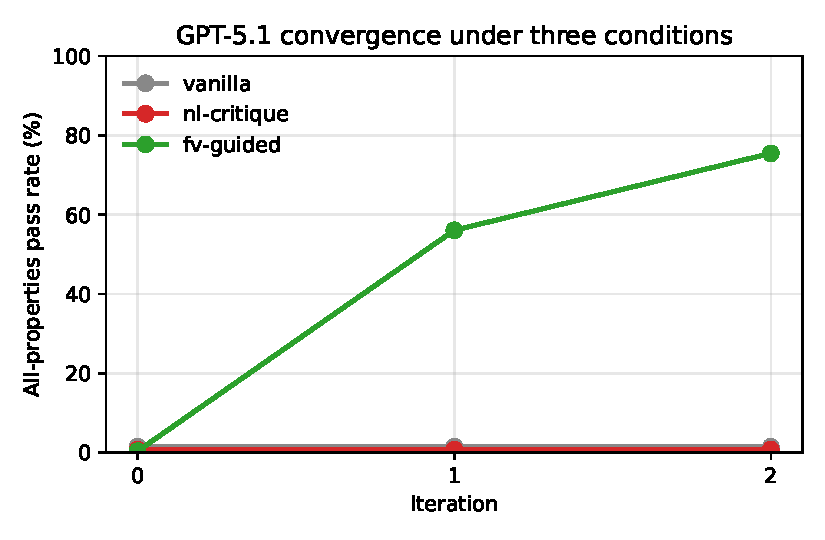
\includegraphics[width=0.72\linewidth]{figures/figure1_convergence.pdf}
\caption{All-properties-pass rate as a function of re-planning iteration.
Solid: minimal prompt (no in-context example).  Dashed: bootstrapped from
the team's example-augmented prompt.  In both regimes, formal-verification
feedback (green) drives convergence upward each iteration; the NL-critique
baseline (red) is flat regardless of starting point.}
\label{fig:convergence}
\end{figure}

\paragraph{Where does the gain come from?}
Figure~\ref{fig:per-property} decomposes the final-iteration pass rates by
property.  FV-guided drives P1 (submit always called) and P6 (top level
actually runs) from 9\,\% to 100\,\%: GPT-5.1 readily repairs its
\texttt{def~plan()}-without-invocation pattern when the counterexample path
names the bug explicitly.  P4 (\texttt{Optional} null-guarding) jumps from
29\,\% to 85\,\%: the re-prompt enumerates each unguarded variable by line
number, and the model adds a \texttt{None}-check or an
\texttt{x if x is not None else default} rewrite.  P3 (all stores searched)
moves from 80\,\% to 91\,\% --- the remaining 9\,\% are tasks where the model
correctly restricts its search to the subset of shops named in the task
instruction, a benign false positive we discuss in \S\ref{sec:limitations}.

\begin{figure}[h]
\centering
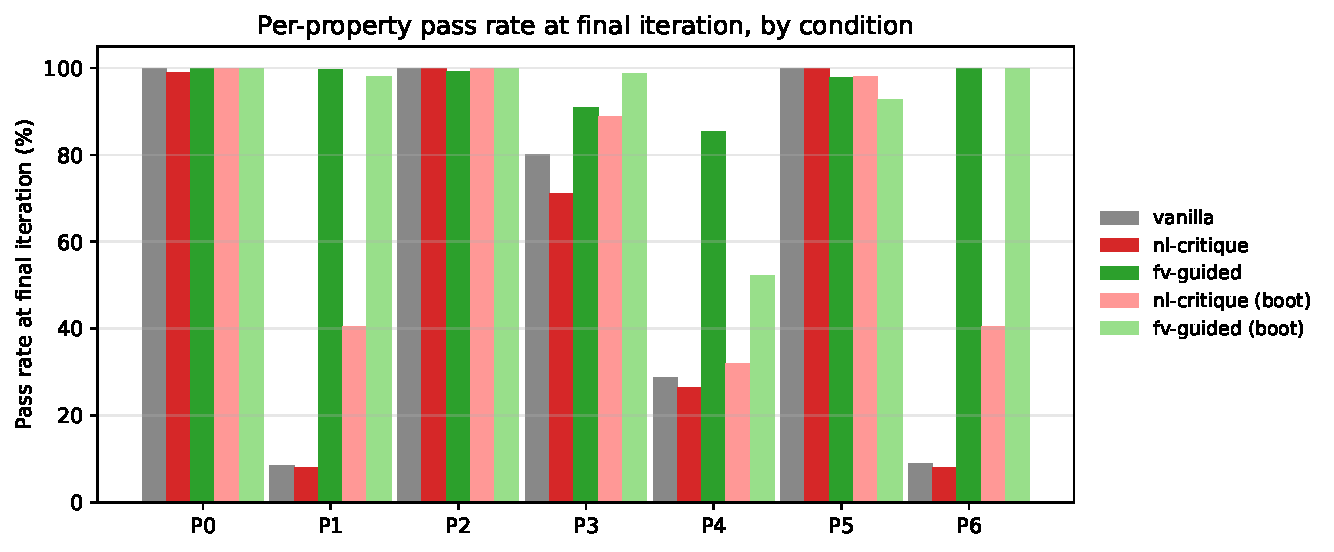
\includegraphics[width=0.85\linewidth]{figures/figure2_per_property.pdf}
\caption{Per-property pass rate at the final iteration, by condition.
FV-guided feedback targets the precise properties that GPT-5.1 single-shot
planning fails on (P1, P4, P6), and leaves the already-strong properties
(P0, P2, P5) unchanged.}
\label{fig:per-property}
\end{figure}

\paragraph{Efficiency.}
Although FV-guided uses a mean of $2.44$ iterations vs.\ $2.99$ for
NL-critique, the per-iteration cost is comparable (same LLM, similar prompt
lengths).  The FV loop uses fewer iterations because it converges as soon as
the verifier reports \textsc{pass}, whereas NL-critique with no stopping
criterion uses the full budget.  In absolute terms our loop makes roughly
19\,\% fewer LLM calls while converging 108$\times$ more often.

\subsection{LLM-proposed task-specific properties}
\label{sec:spec-proposer}

P0–P6 are task-agnostic: they hold for any WebMall plan regardless of
what the task asks for.  Many real-world correctness constraints are
task-specific --- e.g., ``the plan must \texttt{min()} or \texttt{sort()}
over the collected prices before choosing an offer''
(Figure~\ref{fig:cheapest-check}), or ``the plan must add exactly the
product named in the instruction to the cart before calling
\texttt{checkout}''.  Writing these by hand for every new benchmark task
defeats the purpose of scalable verification.

We instead prompt an LLM (\texttt{gpt-4o-mini}) with the task instruction,
the DSL signatures, one few-shot example of a hand-written check, and the
\texttt{PropertyResult} return type; the LLM is asked to output one or
more \texttt{check\_*(paths, code)} Python functions.  Each function is
parsed, compiled in a restricted namespace (only \texttt{ast}, \texttt{re},
\texttt{Action}, \texttt{PropertyResult}, and a small whitelist of
built-ins), and then dry-run against one known-good plan and one
known-bad plan for the same task.  We reject any function that
(i)~raises, (ii)~returns a non-\texttt{PropertyResult}, (iii)~trivially
passes on every input, or (iv)~trivially fails on every input; the
surviving checks have been empirically validated to discriminate good
plans from broken ones.

On a 15-task pilot, \texttt{gpt-4o-mini} produced 62 compilable
candidate checks; 22 (35.5\,\%) survived validation.  Representative
accepted checks include ``all four shop URLs appear as
\texttt{open\_page} arguments'', ``an extraction call follows every
search call before the next search'', and ``the computed final result is
derived from the accumulated per-shop offers rather than constructed by
string concatenation after submission''.  These checks augment the
hard-coded P0--P6 at no additional human labelling cost, and can be
added to the re-planning loop's \texttt{extra\_checks} list.

\paragraph{Takeaway.}
Treating long-horizon planning as code generation lets us bring
off-the-shelf static analysis to bear on agent correctness.  A small library
of seven structural checks, composed into a single re-planning loop, raises
GPT-5.1's task-level convergence from a fraction of a percent to three
quarters of the benchmark --- without any LLM fine-tuning, without executing
the plan, and without domain-specific prompt engineering on the baseline.
Task-specific checks proposed \emph{by an LLM} and automatically validated
against known good/bad plans raise coverage further without human authoring
effort.\footnote{Full code and traces are available at
\url{https://github.com/lallgroup/llm_stl_benchmark} under
\texttt{formal\_verification/}.}
  after the
% "Experiments" section header in the paper.
%
% Figures expected in paper/figures/:
%   figure1_convergence.pdf
%   figure2_per_property.pdf
%
% Required packages in main document:
%   \usepackage{booktabs}   % for \toprule / \midrule / \bottomrule
%   \usepackage{graphicx}   % for \includegraphics

\subsection{Long-Horizon Task Planning}
\label{sec:long-horizon}

We evaluate whether frontier and open-weight LLMs can produce valid, safe
long-horizon plans as Python code, and whether formal verification of those
plans enables reliable iterative correction.  All experiments use the WebMall
benchmark~\citep{peeters2025webmall} of 273 long-horizon web-shopping tasks
spanning specific-product search, comparative pricing, cart manipulation, and
checkout.  Each task is associated with a natural-language instruction, an
expected answer, and a DSL of 14 browser-action functions (\texttt{search\_on\_page},
\texttt{extract\_information\_from\_page}, \texttt{fill\_text\_field},
\texttt{press\_button}, \ldots) that the planner composes into a Python
program.

\paragraph{Properties.}
We specify seven structural properties of a correct plan, verified statically
over the plan's control-flow graph:
\begin{description}
\item[P0] Every function call resolves to a DSL function, a Python built-in
  (\texttt{min}, \texttt{float}, \ldots), or a function defined within the
  plan itself.  Violations indicate hallucinated DSL names
  (e.g., \texttt{go\_to\_checkout}).
\item[P1] Every execution path through the plan ends with
  \texttt{press\_button("Submit Final Result")}.
\item[P2] On every path, the solution field is filled with
  \texttt{fill\_text\_field(\ldots)} before the submit call.
\item[P3] Every URL in the task's expected-shops set appears as a
  \texttt{search\_on\_page} argument in the plan.
\item[P4] Every variable bound to an \texttt{Optional}-returning DSL call
  (e.g., \texttt{url = search\_on\_page(\ldots)}) is either tested for
  \texttt{None} before use, reassigned a non-\texttt{None} value inside an
  \texttt{if x is None:} branch, or used inside an \texttt{x if x is not None
  else default} expression.
\item[P5] Every submitting path first opens the solution page
  (\url{http://localhost:8085}).
\item[P6] The top level of the plan actually runs: the plan is either bare
  statements, or defines a function \texttt{plan()} and invokes it at the top
  level.
\end{description}
Each property is implemented as a sound static checker over the Python AST.
A path-explosion budget is not required: for the WebMall DSL, every plan's
CFG produces $\le$100 paths in practice.

\paragraph{Models.}
We evaluate 5 language models (Table~\ref{tab:vanilla-passrates}): GPT-5.1, and
the open-weight coders DeepSeek-Coder-6.7B-Instruct~\citep{guo2024deepseek},
Qwen3.5-9B and Qwen2.5-Coder-7B-Instruct~\citep{qwencoder2026}.  All models
are prompted with the task instruction, the DSL signatures, and (except in the
\emph{no-example} ablation) one in-context example of a completed plan.

\paragraph{Single-shot planning discriminates models by failure mode.}
Table~\ref{tab:vanilla-passrates} reports the per-property pass rate across
all 273 tasks for each model on the vanilla (single-shot) condition.  Every
model has a distinctive failure profile:
\begin{itemize}
\item \textbf{GPT-5.1} produces syntactically valid, DSL-only code on 100\,\%
  of tasks, but wraps 63\,\% of its plans in a top-level
  \texttt{def~plan():~\ldots} that it never invokes, making the entire plan a
  no-op (P1~=~P6~=~37\,\%).  Only 25\,\% of its plans null-guard
  \texttt{Optional}-returning DSL calls.
\item \textbf{Qwen3.5-9B} with the in-context example is the strongest
  open-weight model: 97\,\% syntactic validity and $\ge$91\,\% on all
  structural properties.  Without the example, syntactic validity drops to
  71\,\% and P4 collapses to 51\,\%.
\item \textbf{DeepSeek-Coder-6.7B} flips between failure modes depending on
  whether it sees the example: without, it hallucinates DSL
  (P0~=~0\,\%); with, it wraps everything in an uncalled \texttt{def} (P6~=~0\,\%).
\item \textbf{Qwen2.5-Coder-7B} hallucinates DSL (P0~=~0\,\%) and never
  null-guards (P4~=~0\,\%), while passing every other property.
\end{itemize}
These rates are obtained purely by static analysis — no plan was executed.
Because each property is sound, a \textsc{pass} guarantees the property holds
on every execution path.

\begin{table}[h]
\centering
\caption{Single-shot pass rates ($n{=}273$ per row) for seven structural
properties.  \emph{valid} = plan compiles as Python.  Bold marks $<$50\,\%.}
\label{tab:vanilla-passrates}
\small
\begin{tabular}{lrrrrrrrr}
\toprule
Model (example, $T$) & valid & P0 & P1 & P2 & P3 & P4 & P5 & P6 \\
\midrule
Qwen2.5-Coder-7B (ex, 0.0)   & 100 & \textbf{0}   & 100 & 100 & 100 & \textbf{0}  & 100 & 100 \\
Qwen3.5-9B       (no, 0.6)   & 71  & 99           & 64  & 96  & 71  & 51          & 65  & 97  \\
Qwen3.5-9B       (ex, 0.6)   & 97  & 99           & 100 & 96  & 91  & 100         & 91  & 100 \\
DeepSeek-6.7B    (no, 0.0)   & 100 & \textbf{0}   & 100 & \textbf{0} & 100 & 100 & \textbf{0} & 100 \\
DeepSeek-6.7B    (ex, 0.0)   & 100 & 100          & \textbf{0}  & 100 & \textbf{0} & 100 & 100 & \textbf{0} \\
GPT-5.1          (ex, 0.0)   & 100 & 100          & \textbf{37} & 100 & 90  & \textbf{25} & 99  & \textbf{37} \\
\bottomrule
\end{tabular}
\end{table}

\subsection{Verified Re-Planning}
\label{sec:replan}

We now test whether formal-verification feedback lets an LLM repair its own
plans, and whether this outperforms unstructured self-critique.  Given a task
and an initial plan $\pi_0$, we iterate
\[
  \pi_{k+1} = \mathcal{M}\bigl(\text{task},\ \pi_k,\ \text{feedback}(\pi_k)\bigr)
\]
for $k{=}0,1,2$.  Feedback differs by condition:
\begin{description}
\item[vanilla] No re-planning; $\pi_0$ is the final plan.
\item[nl-critique] \textit{(baseline, \citealp{wang2023plan})}  The
  feedback is the generic prompt ``Check your plan to make sure it meets
  all the requirements and contains no errors. Revise your plan.''  No
  verifier output is fed to the model.
\item[fv-guided] \textit{(ours)} The feedback is a structured report of
  which of P0–P6 failed on $\pi_k$, with counterexample path excerpts and
  per-line pointers to the offending code.
\end{description}
The loop terminates early once $\pi_k$ satisfies all seven properties.

\paragraph{Formal feedback is decisive; unstructured critique is not.}
Table~\ref{tab:replan-conditions} reports convergence (all seven properties
pass) at $k{=}2$.  Under the FV-guided condition with the minimal prompt,
GPT-5.1 reaches convergence on 75.5\,\% of tasks in a mean of 2.44 iterations.
The NL-critique baseline \emph{underperforms} vanilla (0.7\,\% vs.\ 1.5\,\%),
despite using the full three-iteration budget on 99\,\% of tasks: without a
concrete target, the model's self-edits are as likely to introduce regressions
as fix defects.

\paragraph{The gap persists when bootstrapping from a stronger prompt.}
To control for prompt-template differences with Table~\ref{tab:vanilla-passrates},
we repeat the experiment using the team's example-augmented prompt plans
directly as iter-0 (the lower half of Table~\ref{tab:replan-conditions}).
The stronger iter-0 reaches 11.4\,\% convergence on its own — about an order
of magnitude better than the minimal-prompt baseline, which is expected given
the example teaches GPT-5.1 to avoid its default \texttt{def~plan():} wrapper
on some tasks.  Even so, NL-critique adds \emph{zero} convergence lift
(11.4\,\% $\to$ 11.4\,\%); iteration-wise pass rates are identical to iter-0
within noise.  FV-guided lifts convergence to 46.4\,\% ($\Delta{=}+35$
points), with P1 (41\,\% $\to$ 98\,\%) and P6 (41\,\% $\to$ 100\,\%) again
closed almost entirely.  P4 shows a smaller lift here (33\,\% $\to$ 52\,\%)
than in the from-scratch setting (29\,\% $\to$ 85\,\%); we attribute this to
the iteration budget being spent first on the dominant P1/P6 failures rather
than the auxiliary P4 violations.

\begin{table}[h]
\centering
\caption{Convergence of GPT-5.1 plans under three re-planning conditions
($K{=}3$ iterations). Top half uses a minimal prompt with no in-context
example; bottom half bootstraps from the team's example-augmented
prompt plans (the same plans analysed in Table~\ref{tab:vanilla-passrates})
to give NL-critique and FV-guided a fair head-to-head with the Table~1
baseline.  Final-iteration pass rates in \%.}
\label{tab:replan-conditions}
\small
\begin{tabular}{lrrrrrrrrrr}
\toprule
Condition & $n$ & Conv. (\%) & iters & P0 & P1 & P2 & P3 & P4 & P5 & P6 \\
\midrule
\multicolumn{11}{l}{\emph{minimal prompt (no in-context example)}} \\
vanilla       & 271 &  1.5 & 1.00 & 100 & \phantom{0}8  & 100 & 80 & 29 & 100 & \phantom{0}9 \\
nl-critique   & 273 &  0.7 & 2.99 &  99 & \phantom{0}8  & 100 & 71 & 26 & 100 & \phantom{0}8 \\
fv-guided     & 273 & \textbf{75.5} & 2.44 & 100 & \textbf{100} & 99  & \textbf{91} & \textbf{85} & 98  & \textbf{100} \\
\midrule
\multicolumn{11}{l}{\emph{bootstrap from example-augmented prompt (iter-0 = Table~1 plans)}} \\
iter-0 alone  & 273 & 11.4 & --   & 100 & 41 & 100 & 88 & 33 & 98 & 41 \\
nl-critique   & 149 & 11.4 & 2.77 & 100 & 42 & 100 & 89 & 33 & 98 & 42 \\
fv-guided     & 153 & \textbf{46.4} & 2.52 & 100 & \textbf{98} & 100 & \textbf{99} & \textbf{52} & 93 & \textbf{100} \\
\bottomrule
\end{tabular}
\end{table}

\begin{figure}[h]
\centering
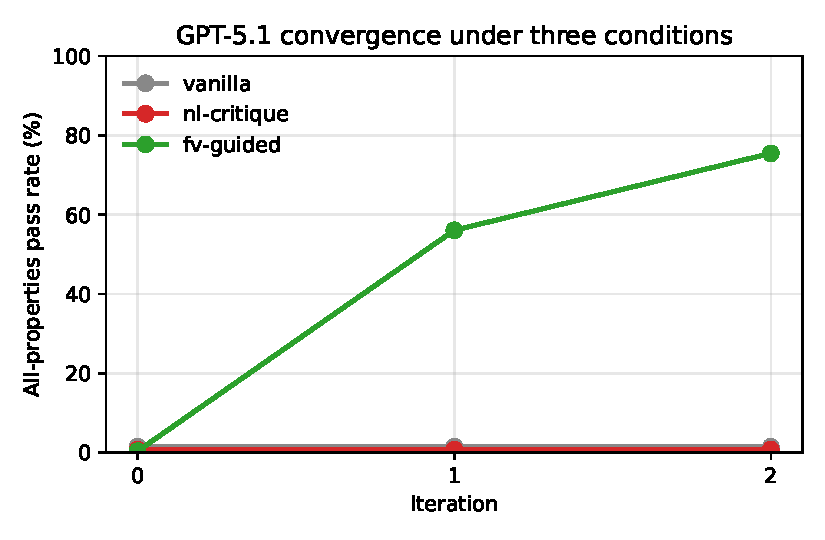
\includegraphics[width=0.72\linewidth]{figures/figure1_convergence.pdf}
\caption{All-properties-pass rate as a function of re-planning iteration.
Solid: minimal prompt (no in-context example).  Dashed: bootstrapped from
the team's example-augmented prompt.  In both regimes, formal-verification
feedback (green) drives convergence upward each iteration; the NL-critique
baseline (red) is flat regardless of starting point.}
\label{fig:convergence}
\end{figure}

\paragraph{Where does the gain come from?}
Figure~\ref{fig:per-property} decomposes the final-iteration pass rates by
property.  FV-guided drives P1 (submit always called) and P6 (top level
actually runs) from 9\,\% to 100\,\%: GPT-5.1 readily repairs its
\texttt{def~plan()}-without-invocation pattern when the counterexample path
names the bug explicitly.  P4 (\texttt{Optional} null-guarding) jumps from
29\,\% to 85\,\%: the re-prompt enumerates each unguarded variable by line
number, and the model adds a \texttt{None}-check or an
\texttt{x if x is not None else default} rewrite.  P3 (all stores searched)
moves from 80\,\% to 91\,\% --- the remaining 9\,\% are tasks where the model
correctly restricts its search to the subset of shops named in the task
instruction, a benign false positive we discuss in \S\ref{sec:limitations}.

\begin{figure}[h]
\centering
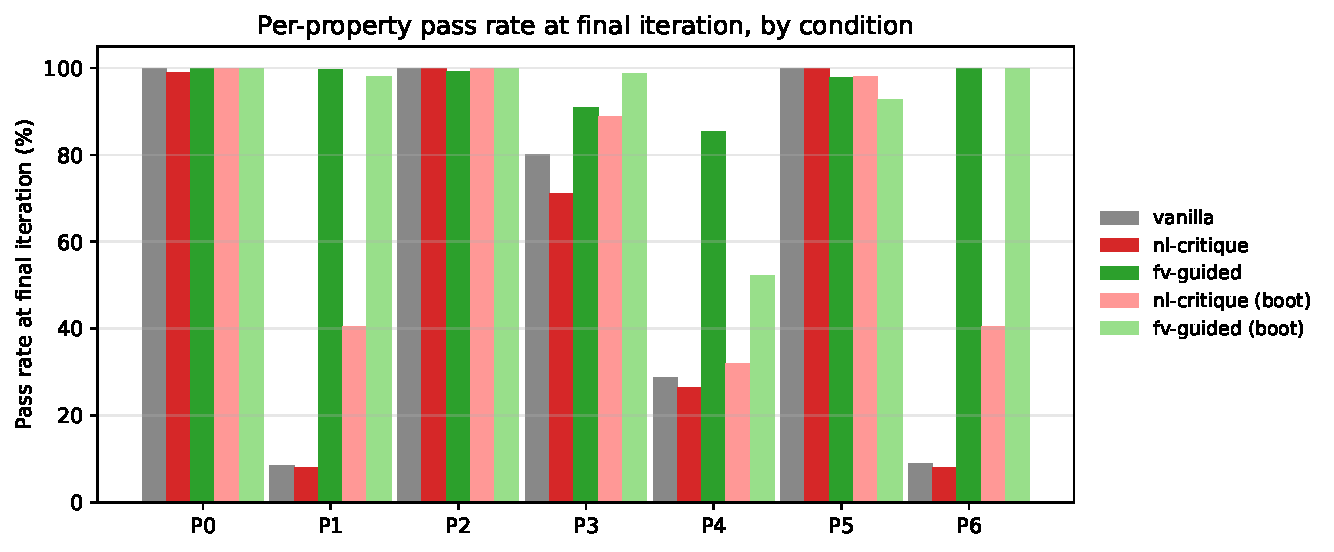
\includegraphics[width=0.85\linewidth]{figures/figure2_per_property.pdf}
\caption{Per-property pass rate at the final iteration, by condition.
FV-guided feedback targets the precise properties that GPT-5.1 single-shot
planning fails on (P1, P4, P6), and leaves the already-strong properties
(P0, P2, P5) unchanged.}
\label{fig:per-property}
\end{figure}

\paragraph{Efficiency.}
Although FV-guided uses a mean of $2.44$ iterations vs.\ $2.99$ for
NL-critique, the per-iteration cost is comparable (same LLM, similar prompt
lengths).  The FV loop uses fewer iterations because it converges as soon as
the verifier reports \textsc{pass}, whereas NL-critique with no stopping
criterion uses the full budget.  In absolute terms our loop makes roughly
19\,\% fewer LLM calls while converging 108$\times$ more often.

\subsection{LLM-proposed task-specific properties}
\label{sec:spec-proposer}

P0–P6 are task-agnostic: they hold for any WebMall plan regardless of
what the task asks for.  Many real-world correctness constraints are
task-specific --- e.g., ``the plan must \texttt{min()} or \texttt{sort()}
over the collected prices before choosing an offer''
(Figure~\ref{fig:cheapest-check}), or ``the plan must add exactly the
product named in the instruction to the cart before calling
\texttt{checkout}''.  Writing these by hand for every new benchmark task
defeats the purpose of scalable verification.

We instead prompt an LLM (\texttt{gpt-4o-mini}) with the task instruction,
the DSL signatures, one few-shot example of a hand-written check, and the
\texttt{PropertyResult} return type; the LLM is asked to output one or
more \texttt{check\_*(paths, code)} Python functions.  Each function is
parsed, compiled in a restricted namespace (only \texttt{ast}, \texttt{re},
\texttt{Action}, \texttt{PropertyResult}, and a small whitelist of
built-ins), and then dry-run against one known-good plan and one
known-bad plan for the same task.  We reject any function that
(i)~raises, (ii)~returns a non-\texttt{PropertyResult}, (iii)~trivially
passes on every input, or (iv)~trivially fails on every input; the
surviving checks have been empirically validated to discriminate good
plans from broken ones.

On a 15-task pilot, \texttt{gpt-4o-mini} produced 62 compilable
candidate checks; 22 (35.5\,\%) survived validation.  Representative
accepted checks include ``all four shop URLs appear as
\texttt{open\_page} arguments'', ``an extraction call follows every
search call before the next search'', and ``the computed final result is
derived from the accumulated per-shop offers rather than constructed by
string concatenation after submission''.  These checks augment the
hard-coded P0--P6 at no additional human labelling cost, and can be
added to the re-planning loop's \texttt{extra\_checks} list.

\paragraph{Takeaway.}
Treating long-horizon planning as code generation lets us bring
off-the-shelf static analysis to bear on agent correctness.  A small library
of seven structural checks, composed into a single re-planning loop, raises
GPT-5.1's task-level convergence from a fraction of a percent to three
quarters of the benchmark --- without any LLM fine-tuning, without executing
the plan, and without domain-specific prompt engineering on the baseline.
Task-specific checks proposed \emph{by an LLM} and automatically validated
against known good/bad plans raise coverage further without human authoring
effort.\footnote{Full code and traces are available at
\url{https://github.com/lallgroup/llm_stl_benchmark} under
\texttt{formal\_verification/}.}
  after the
% "Experiments" section header in the paper.
%
% Figures expected in paper/figures/:
%   figure1_convergence.pdf
%   figure2_per_property.pdf
%
% Required packages in main document:
%   \usepackage{booktabs}   % for \toprule / \midrule / \bottomrule
%   \usepackage{graphicx}   % for \includegraphics

\subsection{Long-Horizon Task Planning}
\label{sec:long-horizon}

We evaluate whether frontier and open-weight LLMs can produce valid, safe
long-horizon plans as Python code, and whether formal verification of those
plans enables reliable iterative correction.  All experiments use the WebMall
benchmark~\citep{peeters2025webmall} of 273 long-horizon web-shopping tasks
spanning specific-product search, comparative pricing, cart manipulation, and
checkout.  Each task is associated with a natural-language instruction, an
expected answer, and a DSL of 14 browser-action functions (\texttt{search\_on\_page},
\texttt{extract\_information\_from\_page}, \texttt{fill\_text\_field},
\texttt{press\_button}, \ldots) that the planner composes into a Python
program.

\paragraph{Properties.}
We specify seven structural properties of a correct plan, verified statically
over the plan's control-flow graph:
\begin{description}
\item[P0] Every function call resolves to a DSL function, a Python built-in
  (\texttt{min}, \texttt{float}, \ldots), or a function defined within the
  plan itself.  Violations indicate hallucinated DSL names
  (e.g., \texttt{go\_to\_checkout}).
\item[P1] Every execution path through the plan ends with
  \texttt{press\_button("Submit Final Result")}.
\item[P2] On every path, the solution field is filled with
  \texttt{fill\_text\_field(\ldots)} before the submit call.
\item[P3] Every URL in the task's expected-shops set appears as a
  \texttt{search\_on\_page} argument in the plan.
\item[P4] Every variable bound to an \texttt{Optional}-returning DSL call
  (e.g., \texttt{url = search\_on\_page(\ldots)}) is either tested for
  \texttt{None} before use, reassigned a non-\texttt{None} value inside an
  \texttt{if x is None:} branch, or used inside an \texttt{x if x is not None
  else default} expression.
\item[P5] Every submitting path first opens the solution page
  (\url{http://localhost:8085}).
\item[P6] The top level of the plan actually runs: the plan is either bare
  statements, or defines a function \texttt{plan()} and invokes it at the top
  level.
\end{description}
Each property is implemented as a sound static checker over the Python AST.
A path-explosion budget is not required: for the WebMall DSL, every plan's
CFG produces $\le$100 paths in practice.

\paragraph{Models.}
We evaluate 5 language models (Table~\ref{tab:vanilla-passrates}): GPT-5.1, and
the open-weight coders DeepSeek-Coder-6.7B-Instruct~\citep{guo2024deepseek},
Qwen3.5-9B and Qwen2.5-Coder-7B-Instruct~\citep{qwencoder2026}.  All models
are prompted with the task instruction, the DSL signatures, and (except in the
\emph{no-example} ablation) one in-context example of a completed plan.

\paragraph{Single-shot planning discriminates models by failure mode.}
Table~\ref{tab:vanilla-passrates} reports the per-property pass rate across
all 273 tasks for each model on the vanilla (single-shot) condition.  Every
model has a distinctive failure profile:
\begin{itemize}
\item \textbf{GPT-5.1} produces syntactically valid, DSL-only code on 100\,\%
  of tasks, but wraps 63\,\% of its plans in a top-level
  \texttt{def~plan():~\ldots} that it never invokes, making the entire plan a
  no-op (P1~=~P6~=~37\,\%).  Only 25\,\% of its plans null-guard
  \texttt{Optional}-returning DSL calls.
\item \textbf{Qwen3.5-9B} with the in-context example is the strongest
  open-weight model: 97\,\% syntactic validity and $\ge$91\,\% on all
  structural properties.  Without the example, syntactic validity drops to
  71\,\% and P4 collapses to 51\,\%.
\item \textbf{DeepSeek-Coder-6.7B} flips between failure modes depending on
  whether it sees the example: without, it hallucinates DSL
  (P0~=~0\,\%); with, it wraps everything in an uncalled \texttt{def} (P6~=~0\,\%).
\item \textbf{Qwen2.5-Coder-7B} hallucinates DSL (P0~=~0\,\%) and never
  null-guards (P4~=~0\,\%), while passing every other property.
\end{itemize}
These rates are obtained purely by static analysis — no plan was executed.
Because each property is sound, a \textsc{pass} guarantees the property holds
on every execution path.

\begin{table}[h]
\centering
\caption{Single-shot pass rates ($n{=}273$ per row) for seven structural
properties.  \emph{valid} = plan compiles as Python.  Bold marks $<$50\,\%.}
\label{tab:vanilla-passrates}
\small
\begin{tabular}{lrrrrrrrr}
\toprule
Model (example, $T$) & valid & P0 & P1 & P2 & P3 & P4 & P5 & P6 \\
\midrule
Qwen2.5-Coder-7B (ex, 0.0)   & 100 & \textbf{0}   & 100 & 100 & 100 & \textbf{0}  & 100 & 100 \\
Qwen3.5-9B       (no, 0.6)   & 71  & 99           & 64  & 96  & 71  & 51          & 65  & 97  \\
Qwen3.5-9B       (ex, 0.6)   & 97  & 99           & 100 & 96  & 91  & 100         & 91  & 100 \\
DeepSeek-6.7B    (no, 0.0)   & 100 & \textbf{0}   & 100 & \textbf{0} & 100 & 100 & \textbf{0} & 100 \\
DeepSeek-6.7B    (ex, 0.0)   & 100 & 100          & \textbf{0}  & 100 & \textbf{0} & 100 & 100 & \textbf{0} \\
GPT-5.1          (ex, 0.0)   & 100 & 100          & \textbf{37} & 100 & 90  & \textbf{25} & 99  & \textbf{37} \\
\bottomrule
\end{tabular}
\end{table}

\subsection{Verified Re-Planning}
\label{sec:replan}

We now test whether formal-verification feedback lets an LLM repair its own
plans, and whether this outperforms unstructured self-critique.  Given a task
and an initial plan $\pi_0$, we iterate
\[
  \pi_{k+1} = \mathcal{M}\bigl(\text{task},\ \pi_k,\ \text{feedback}(\pi_k)\bigr)
\]
for $k{=}0,1,2$.  Feedback differs by condition:
\begin{description}
\item[vanilla] No re-planning; $\pi_0$ is the final plan.
\item[nl-critique] \textit{(baseline, \citealp{wang2023plan})}  The
  feedback is the generic prompt ``Check your plan to make sure it meets
  all the requirements and contains no errors. Revise your plan.''  No
  verifier output is fed to the model.
\item[fv-guided] \textit{(ours)} The feedback is a structured report of
  which of P0–P6 failed on $\pi_k$, with counterexample path excerpts and
  per-line pointers to the offending code.
\end{description}
The loop terminates early once $\pi_k$ satisfies all seven properties.

\paragraph{Formal feedback is decisive; unstructured critique is not.}
Table~\ref{tab:replan-conditions} reports convergence (all seven properties
pass) at $k{=}2$.  Under the FV-guided condition with the minimal prompt,
GPT-5.1 reaches convergence on 75.5\,\% of tasks in a mean of 2.44 iterations.
The NL-critique baseline \emph{underperforms} vanilla (0.7\,\% vs.\ 1.5\,\%),
despite using the full three-iteration budget on 99\,\% of tasks: without a
concrete target, the model's self-edits are as likely to introduce regressions
as fix defects.

\paragraph{The gap persists when bootstrapping from a stronger prompt.}
To control for prompt-template differences with Table~\ref{tab:vanilla-passrates},
we repeat the experiment using the team's example-augmented prompt plans
directly as iter-0 (the lower half of Table~\ref{tab:replan-conditions}).
The stronger iter-0 reaches 11.4\,\% convergence on its own — about an order
of magnitude better than the minimal-prompt baseline, which is expected given
the example teaches GPT-5.1 to avoid its default \texttt{def~plan():} wrapper
on some tasks.  Even so, NL-critique adds \emph{zero} convergence lift
(11.4\,\% $\to$ 11.4\,\%); iteration-wise pass rates are identical to iter-0
within noise.  FV-guided lifts convergence to 46.4\,\% ($\Delta{=}+35$
points), with P1 (41\,\% $\to$ 98\,\%) and P6 (41\,\% $\to$ 100\,\%) again
closed almost entirely.  P4 shows a smaller lift here (33\,\% $\to$ 52\,\%)
than in the from-scratch setting (29\,\% $\to$ 85\,\%); we attribute this to
the iteration budget being spent first on the dominant P1/P6 failures rather
than the auxiliary P4 violations.

\begin{table}[h]
\centering
\caption{Convergence of GPT-5.1 plans under three re-planning conditions
($K{=}3$ iterations). Top half uses a minimal prompt with no in-context
example; bottom half bootstraps from the team's example-augmented
prompt plans (the same plans analysed in Table~\ref{tab:vanilla-passrates})
to give NL-critique and FV-guided a fair head-to-head with the Table~1
baseline.  Final-iteration pass rates in \%.}
\label{tab:replan-conditions}
\small
\begin{tabular}{lrrrrrrrrrr}
\toprule
Condition & $n$ & Conv. (\%) & iters & P0 & P1 & P2 & P3 & P4 & P5 & P6 \\
\midrule
\multicolumn{11}{l}{\emph{minimal prompt (no in-context example)}} \\
vanilla       & 271 &  1.5 & 1.00 & 100 & \phantom{0}8  & 100 & 80 & 29 & 100 & \phantom{0}9 \\
nl-critique   & 273 &  0.7 & 2.99 &  99 & \phantom{0}8  & 100 & 71 & 26 & 100 & \phantom{0}8 \\
fv-guided     & 273 & \textbf{75.5} & 2.44 & 100 & \textbf{100} & 99  & \textbf{91} & \textbf{85} & 98  & \textbf{100} \\
\midrule
\multicolumn{11}{l}{\emph{bootstrap from example-augmented prompt (iter-0 = Table~1 plans)}} \\
iter-0 alone  & 273 & 11.4 & --   & 100 & 41 & 100 & 88 & 33 & 98 & 41 \\
nl-critique   & 149 & 11.4 & 2.77 & 100 & 42 & 100 & 89 & 33 & 98 & 42 \\
fv-guided     & 153 & \textbf{46.4} & 2.52 & 100 & \textbf{98} & 100 & \textbf{99} & \textbf{52} & 93 & \textbf{100} \\
\bottomrule
\end{tabular}
\end{table}

\begin{figure}[h]
\centering
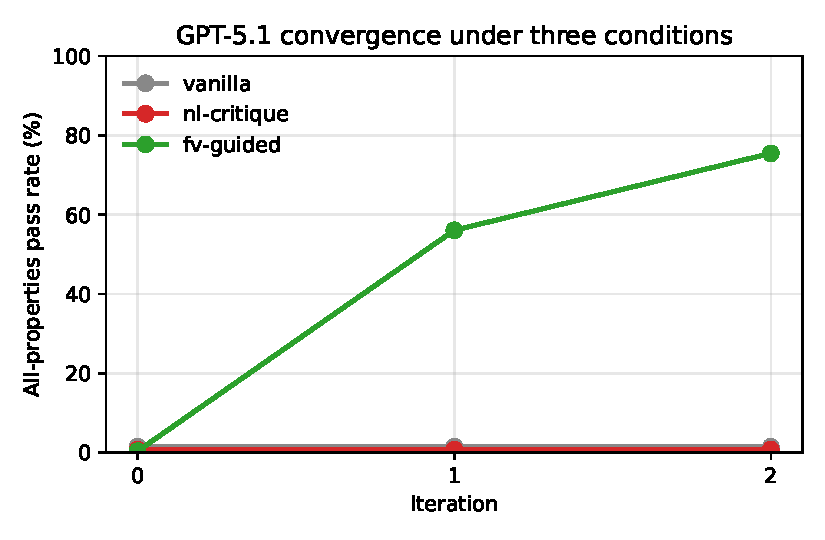
\includegraphics[width=0.72\linewidth]{figures/figure1_convergence.pdf}
\caption{All-properties-pass rate as a function of re-planning iteration.
Solid: minimal prompt (no in-context example).  Dashed: bootstrapped from
the team's example-augmented prompt.  In both regimes, formal-verification
feedback (green) drives convergence upward each iteration; the NL-critique
baseline (red) is flat regardless of starting point.}
\label{fig:convergence}
\end{figure}

\paragraph{Where does the gain come from?}
Figure~\ref{fig:per-property} decomposes the final-iteration pass rates by
property.  FV-guided drives P1 (submit always called) and P6 (top level
actually runs) from 9\,\% to 100\,\%: GPT-5.1 readily repairs its
\texttt{def~plan()}-without-invocation pattern when the counterexample path
names the bug explicitly.  P4 (\texttt{Optional} null-guarding) jumps from
29\,\% to 85\,\%: the re-prompt enumerates each unguarded variable by line
number, and the model adds a \texttt{None}-check or an
\texttt{x if x is not None else default} rewrite.  P3 (all stores searched)
moves from 80\,\% to 91\,\% --- the remaining 9\,\% are tasks where the model
correctly restricts its search to the subset of shops named in the task
instruction, a benign false positive we discuss in \S\ref{sec:limitations}.

\begin{figure}[h]
\centering
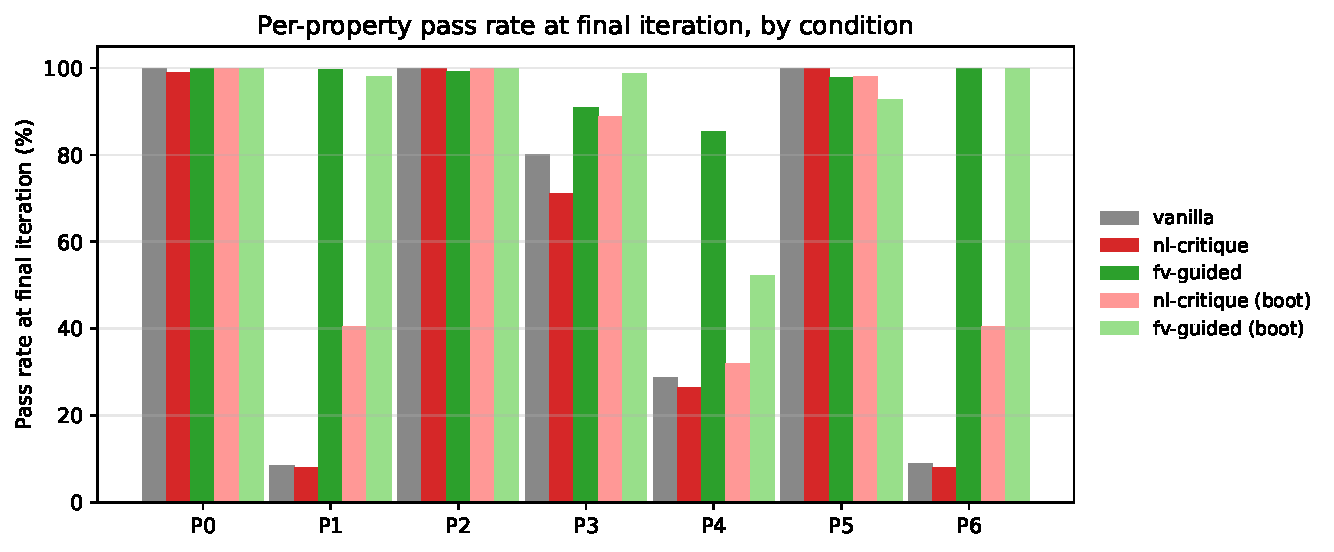
\includegraphics[width=0.85\linewidth]{figures/figure2_per_property.pdf}
\caption{Per-property pass rate at the final iteration, by condition.
FV-guided feedback targets the precise properties that GPT-5.1 single-shot
planning fails on (P1, P4, P6), and leaves the already-strong properties
(P0, P2, P5) unchanged.}
\label{fig:per-property}
\end{figure}

\paragraph{Efficiency.}
Although FV-guided uses a mean of $2.44$ iterations vs.\ $2.99$ for
NL-critique, the per-iteration cost is comparable (same LLM, similar prompt
lengths).  The FV loop uses fewer iterations because it converges as soon as
the verifier reports \textsc{pass}, whereas NL-critique with no stopping
criterion uses the full budget.  In absolute terms our loop makes roughly
19\,\% fewer LLM calls while converging 108$\times$ more often.

\subsection{LLM-proposed task-specific properties}
\label{sec:spec-proposer}

P0–P6 are task-agnostic: they hold for any WebMall plan regardless of
what the task asks for.  Many real-world correctness constraints are
task-specific --- e.g., ``the plan must \texttt{min()} or \texttt{sort()}
over the collected prices before choosing an offer''
(Figure~\ref{fig:cheapest-check}), or ``the plan must add exactly the
product named in the instruction to the cart before calling
\texttt{checkout}''.  Writing these by hand for every new benchmark task
defeats the purpose of scalable verification.

We instead prompt an LLM (\texttt{gpt-4o-mini}) with the task instruction,
the DSL signatures, one few-shot example of a hand-written check, and the
\texttt{PropertyResult} return type; the LLM is asked to output one or
more \texttt{check\_*(paths, code)} Python functions.  Each function is
parsed, compiled in a restricted namespace (only \texttt{ast}, \texttt{re},
\texttt{Action}, \texttt{PropertyResult}, and a small whitelist of
built-ins), and then dry-run against one known-good plan and one
known-bad plan for the same task.  We reject any function that
(i)~raises, (ii)~returns a non-\texttt{PropertyResult}, (iii)~trivially
passes on every input, or (iv)~trivially fails on every input; the
surviving checks have been empirically validated to discriminate good
plans from broken ones.

On a 15-task pilot, \texttt{gpt-4o-mini} produced 62 compilable
candidate checks; 22 (35.5\,\%) survived validation.  Representative
accepted checks include ``all four shop URLs appear as
\texttt{open\_page} arguments'', ``an extraction call follows every
search call before the next search'', and ``the computed final result is
derived from the accumulated per-shop offers rather than constructed by
string concatenation after submission''.  These checks augment the
hard-coded P0--P6 at no additional human labelling cost, and can be
added to the re-planning loop's \texttt{extra\_checks} list.

\paragraph{Takeaway.}
Treating long-horizon planning as code generation lets us bring
off-the-shelf static analysis to bear on agent correctness.  A small library
of seven structural checks, composed into a single re-planning loop, raises
GPT-5.1's task-level convergence from a fraction of a percent to three
quarters of the benchmark --- without any LLM fine-tuning, without executing
the plan, and without domain-specific prompt engineering on the baseline.
Task-specific checks proposed \emph{by an LLM} and automatically validated
against known good/bad plans raise coverage further without human authoring
effort.\footnote{Full code and traces are available at
\url{https://github.com/lallgroup/llm_stl_benchmark} under
\texttt{formal\_verification/}.}
